\begin{figure}[H]
    \begin{subfigure}{0.4\linewidth}
        \centering
        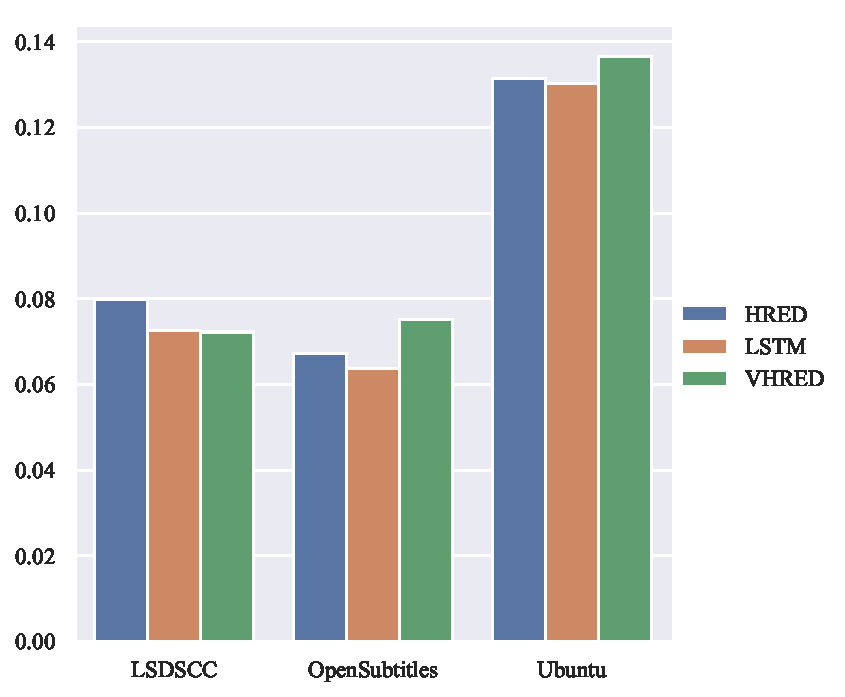
\includegraphics[width=\linewidth]{figure/barplot/bleu_1/plot.pdf}
        \caption{BLEU-1}
    \end{subfigure}%
    \begin{subfigure}{0.4\linewidth}
        \centering
        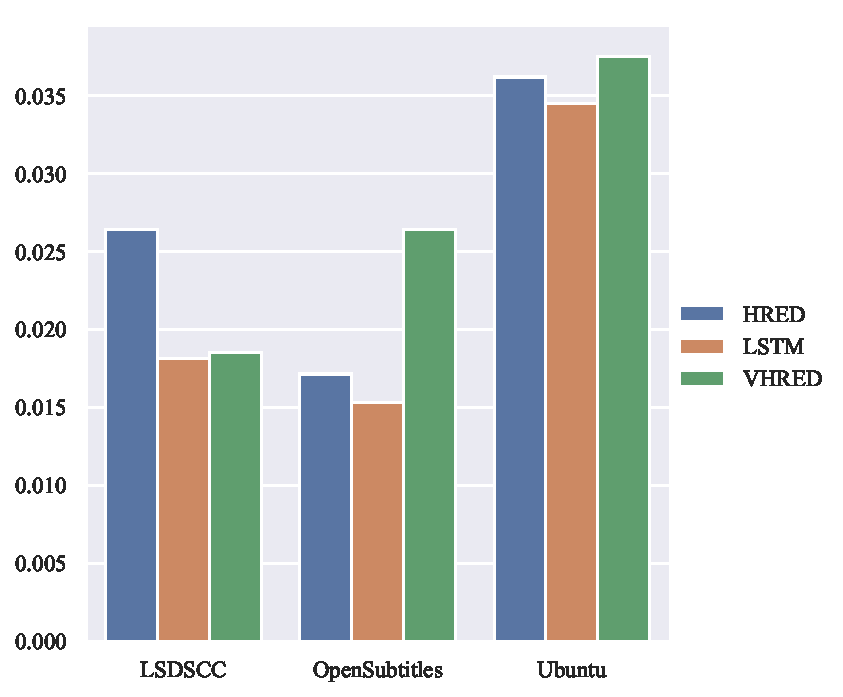
\includegraphics[width=\linewidth]{figure/barplot/bleu_2/plot.pdf}
        \caption{BLEU-2}
    \end{subfigure}
    \begin{subfigure}{0.4\linewidth}
        \centering
        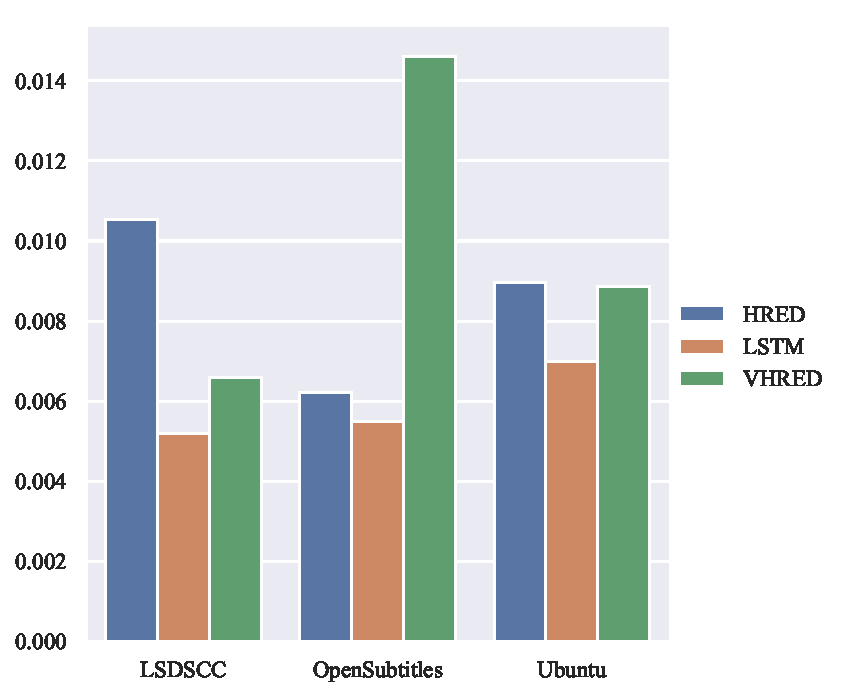
\includegraphics[width=\linewidth]{figure/barplot/bleu_3/plot.pdf}
        \caption{BLEU-3}
    \end{subfigure}%
    \begin{subfigure}{0.4\linewidth}
        \centering
        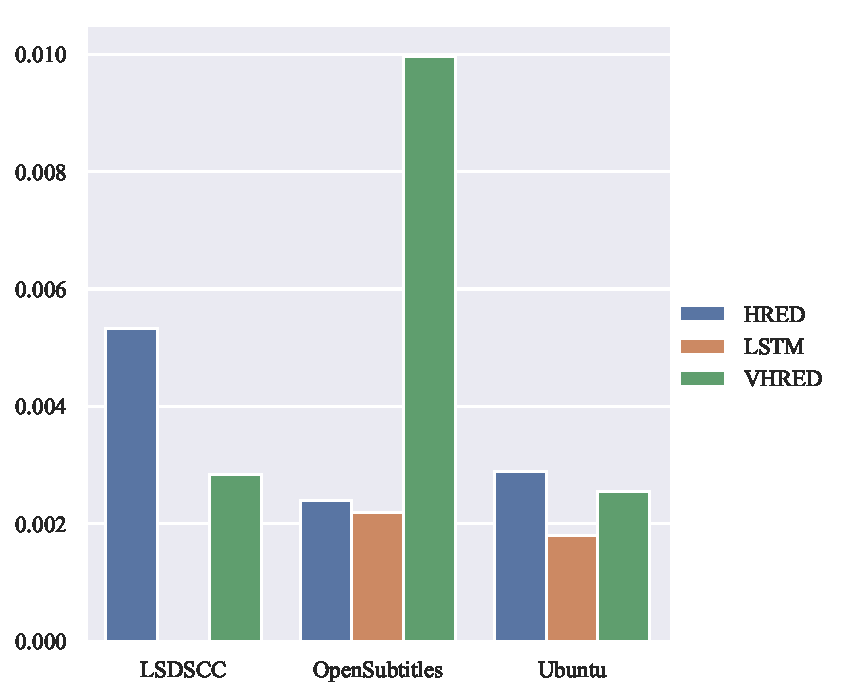
\includegraphics[width=\linewidth]{figure/barplot/bleu_4/plot.pdf}
        \caption{BLEU-4}
    \end{subfigure}
    \centering
    \caption{BLEU的系统得分}
    \label{fig:BLEU_system}
\end{figure}
